\documentclass{standalone}
\usepackage{tikz}
\usetikzlibrary{arrows.meta, positioning, shapes.multipart, calc}

\begin{document}
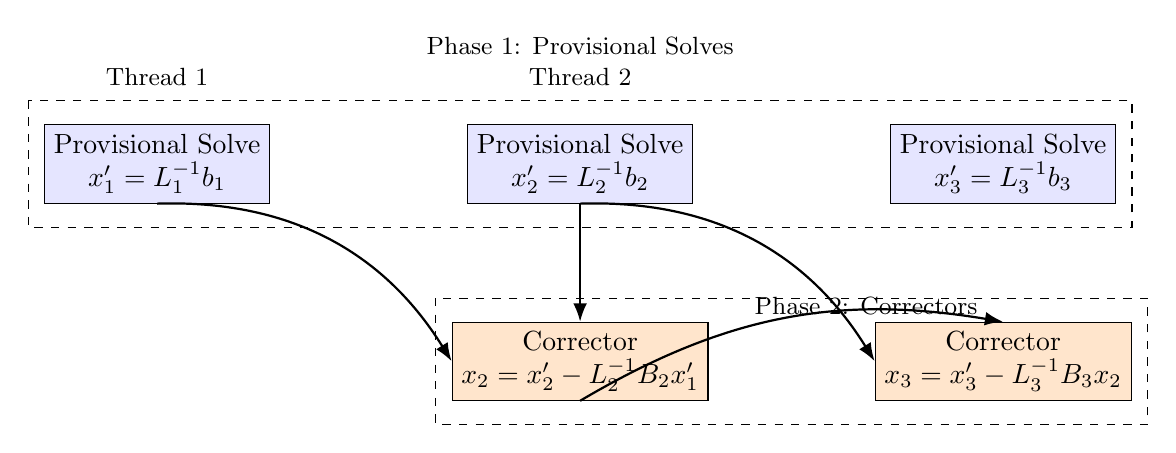
\begin{tikzpicture}[
    task/.style={rectangle, draw, fill=blue!10, minimum width=2.5cm, minimum height=0.9cm, align=center},
    corr/.style={rectangle, draw, fill=orange!20, minimum width=3cm, minimum height=0.9cm, align=center},
    dep/.style={-Latex, thick},
    dasheddep/.style={-Latex, thick, dashed},
    label/.style={font=\small}
]

% Task nodes for provisional solves (x'_i)
\node[task] (x1) at (0,0) {Provisional Solve \\ $x'_1 = L_1^{-1}b_1$};
\node[task] (x2) [right=2.5cm of x1] {Provisional Solve \\ $x'_2 = L_2^{-1}b_2$};
\node[task] (x3) [right=2.5cm of x2] {Provisional Solve \\ $x'_3 = L_3^{-1}b_3$};

% Corrector nodes
\node[corr] (c2) [below=1.5cm of x2] {Corrector \\ $x_2 = x'_2 - L_2^{-1}B_2x'_1$};
\node[corr] (c3) [below=1.5cm of x3] {Corrector \\ $x_3 = x'_3 - L_3^{-1}B_3x_2$};

% Dependencies
\draw[dep] (x1.south) to[bend left=30] (c2.west);
\draw[dep] (x2.south) -- (c2.north);

\draw[dep] (x2.south) to[bend left=30] (c3.west);
\draw[dep] (c2.south) to[bend left=20] (c3.north);

% Optional labels for threads
\node[label] at ($(x1.north)+(0,0.6)$) {Thread 1};
\node[label] at ($(x2.north)+(0,0.6)$) {Thread 2};

% Optional bracket for phase 1
\draw[dashed] ($(x1.north west)+(-0.2,0.3)$) rectangle ($(x3.south east)+(0.2,-0.3)$);
\node[label] at ($(x2.north)+(0,1)$) {Phase 1: Provisional Solves};

% Optional bracket for phase 2
\draw[dashed] ($(c2.north west)+(-0.2,0.3)$) rectangle ($(c3.south east)+(0.2,-0.3)$);
\node[label] at ($(c2.north east)+(2,0.2)$) {Phase 2: Correctors};

\end{tikzpicture}
\end{document}
